\section{Estimates for large $x$}\label{initial-sec}

We can now begin the proof of Theorem \ref{eff}.  
The strategy is to use the expansion \eqref{htz-expand}, which turns out to be an effective approximation in the region \eqref{region}, since we will be able to ensure that quantities such as $s + \sqrt{t} v + \frac{t}{2} \alpha_n$ or $s + \sqrt{t} v + \frac{t}{2} \beta_N$, with $s = \frac{1+i(x+iy)}{2}$, stay away from the real axis where the poles of $\Gamma$ are located (and also where the error terms in the Riemann-Siegel approximation deteriorate).  

Accordingly, we will need effective estimates on the functions $r_{t,n}, R_{t,N}$ appearing in Section \ref{heatflow-sec}.  We will treat these two functions separately.

\subsection{Estimation of $r_{t,n}$}

We recall the function $\alpha(s)$ defined in \eqref{alpha-def}.  From differentiating \eqref{alpha-form} we see that
\begin{equation}\label{alpha-deriv}
 \alpha'(s) = -\frac{1}{2s^2} - \frac{1}{(s-1)^2} + \frac{1}{2 s}
\end{equation}
whenever $s \in \C \backslash (-\infty,1]$.  If $\mathrm{Im}(s) > 3$, we conclude in particular the useful bound
\begin{equation}\label{alpha-deriv-bound}
\begin{split}
 \alpha'(s) &= O_{\leq}\left( \frac{1}{2\Im(s)^2} \right) + O_{\leq}\left( \frac{1}{\Im(s)^2} \right) + O_{\leq}\left( \frac{1}{2\Im(s)} \right) \\
 &= O_{\leq}\left( \frac{1}{2 \Im(s)-6} \right)
\end{split}
\end{equation}
thanks to Lemma \ref{elem-lem}(i).  

We also recall the function $M_t$ and the coefficients $b_n^t$ from \eqref{Mt-def}, \eqref{bn-def} respectively.  It turns out we have a good approximation
$$r_{t,n}(\sigma+iT) \approx M_t(\sigma+iT) \frac{b_n^t}{n^{\sigma+iT+\frac{t}{2} \alpha(\sigma+iT)}}.$$
More precisely, we have

\begin{proposition}[Estimate for $r_{t,n}$]\label{rtn-prop}  Let $\sigma$ be real, let $T>10$, let $n$ be a positive integer, and let $0 < t \leq 1/2$.  Then 
$$ r_{t,n}(\sigma+iT) = M_t(\sigma+iT) \frac{b_n^t}{n^{\sigma+iT+\frac{t}{2} \alpha(\sigma+iT)}} \left(1 + O_{\leq}(\eps_{t,n}(\sigma+iT))\right)$$
where 
\begin{equation}\label{eps-def}
 \eps_{t,n}(\sigma+iT) \coloneqq \exp\left( \frac{\frac{t^2}{8} |\alpha(\sigma+iT) - \log n|^2 + \frac{t}{4} + \frac{1}{6}}{T-3.33} \right)-1.
\end{equation}
\end{proposition}

\begin{proof}  From \eqref{ron-def}, \eqref{M-def} and Lemma \ref{elem-lem}(v) one has
$$ 
r_{0,n}(s) = M_0(s) n^{-s} \exp\left( O_{\leq}\left( \frac{1}{6(|s|-0.66)} \right) \right)
$$
whenever $\mathrm{Im}(s) > 2$.  Let $\alpha_n$ denote the quantity
\begin{equation}\label{alphan-def}
\alpha_n \coloneqq \alpha(\sigma+iT) - \log n;
\end{equation}
this is the logarithmic derivative of $M(s) n^{-s}$ at $s=\sigma+iT$.  
By \eqref{alpha-form} and the hypothesis $T \geq 10$, the imaginary part of $\alpha_n$ may be lower bounded by
\begin{equation}\label{iman}
 \mathrm{Im}(\alpha_n) \geq -\frac{1}{2T} - \frac{1}{T} \geq -0.15;
\end{equation}
in particular, $\sigma+iT$ and $\sigma+iT+\frac{t}{2}\alpha_n$ have imaginary parts of the same sign.
We can now apply \eqref{rtn-def} to obtain
\begin{align*}
 r_{t,n}(\sigma+iT) &= \exp\left( - \frac{t}{4} \alpha_n^2\right) \int_\R \exp\left( - \sqrt{t} v \alpha_n\right) M_0\left( \sigma + iT + \sqrt{t} v + \frac{t}{2} \alpha_n\right) \times \\
&\quad \times \exp\left( -\left(\sigma+iT+\sqrt{t} v + \frac{t}{2} \alpha_n \right) \log n + O_{\leq}\left( \frac{1}{6(|\sigma+iT+\sqrt{t} v + \frac{t}{2} \alpha_n|-0.66)} \right) \right)
\frac{1}{\sqrt{\pi}} e^{-v^2}\ dv.
\end{align*}
From \eqref{iman} we see that $\sigma+iT+\sqrt{t}v+\frac{t}{2}\alpha_n)$ has imaginary part at least $T-0.08$. Thus
$$ O_{\leq}\left( \frac{1}{6(|\sigma+iT+\sqrt{t} v + \frac{t}{2} \alpha_n|-0.66)} \right)  = 
O_{\leq}\left( \frac{1}{6(T - 0.74)} \right) = O_{\leq}\left( \frac{1}{6(T - 3.08)} \right).$$
From \eqref{alpha-deriv-bound} we have
$$ \alpha'(s) = O_{\leq}\left( \frac{1}{2(T-3.08)} \right)$$
for all $s$ on the line segment between $\sigma+iT$ and $\sigma + iT + \sqrt{t} v + \frac{t}{2} \alpha_n$.  Applying Taylor's theorem with remainder to the branch of the logarithm $\log M_0$ defined in \eqref{logM}, we conclude that
$$ M_0( \sigma + iT + \sqrt{t} v + \frac{t}{2} \alpha_n) = M_0(\sigma+iT) \exp\left( \alpha(\sigma+iT) (\sqrt{t} v + \frac{t}{2} \alpha_n) + O_{\leq}\left( \frac{|\sqrt{t} v + \frac{t}{2} \alpha_n|^2}{4(T-3.08)}  \right)\right).$$
Combining these estimates, writing $\alpha(\sigma+iT) = \alpha_n + \log n$, estimating $|\sqrt{t} v + \frac{t}{2} \alpha_n|^2$ by $2tv^2 + \frac{t^2}{2} |\alpha_n|^2$, and simplifying, we conclude that
\begin{align*}
 r_{t,n}(s) &= M_0(\sigma+iT) \exp\left( \frac{t}{4} \alpha_n^2 - (\sigma+iT) \log n\right) \times \\
&\quad \times  \int_\R \exp\left(  O_{\leq}\left( \frac{\frac{t}{2}v^2 + \frac{t^2}{8} |\alpha_n|^2 + \frac{1}{6}}{T-3.08} \right) \right) \frac{1}{\sqrt{\pi}} e^{-v^2}\ dv.
\end{align*}
Using \eqref{alphan-def}, \eqref{Mt-def}, \eqref{bn-def} we see that
$$ M_0(\sigma+iT) \exp\left( \frac{t}{4} \alpha_n^2 - (\sigma+iT) \log n\right) = M_t(\sigma+iT) \frac{b_n^t}{n^{\sigma+iT+\frac{t}{2} \alpha(\sigma+iT)}} $$
and so it suffices to show that
$$  \int_\R \exp\left( O_{\leq}\left( \frac{\frac{t}{2}v^2 + \frac{t^2}{8} |\alpha_n|^2 + \frac{1}{6}}{T-3.08} \right) \right)\frac{1}{\sqrt{\pi}} e^{-v^2}\ dv = 1 + O\left(\exp\left( \frac{\frac{t^2}{8} |\alpha_n|^2 + \frac{t}{4} + \frac{1}{6}}{T-3.33} \right)-1\right).$$
Since $\frac{1}{\sqrt{\pi}} e^{-v^2}\ dv $ integrates to one, it suffices by Lemma \ref{elem-lem}(iv) to show that
$$
  \int_\R \exp\left( \frac{t v^2+ \frac{t^2}{8} |\alpha_n|^2 + \frac{1}{6}}{2(T-3.08)} \right) \frac{1}{\sqrt{\pi}} e^{-v^2}\ dv \leq \exp\left( \frac{\frac{t^2}{8} |\alpha_n|^2 + \frac{t}{4} + \frac{1}{6}}{T-3.33} \right).
$$
Since $\frac{1}{T-3.08} < \frac{1}{T-3.33}$, we can remove the $\frac{t^2}{8} |\alpha_n|^2 + \frac{1}{6}$ terms from both sides and reduce to showing that
\begin{equation}\label{ax}
  \int_\R \exp\left( \frac{t v^2}{2(T-3.08)} \right) \frac{1}{\sqrt{\pi}} e^{-v^2}\ dv \leq \exp\left( \frac{t}{4(T-3.33)} \right).
	\end{equation}
Using \eqref{gaussian}, the left-hand side may be calculated exactly as
$$ \left(1 - \frac{t}{2(T-3.08)}\right)^{-1/2}.$$
Applying Lemma \ref{elem-lem}(ii) and using the hypotheses $t \leq 1/2$, $T \geq 10$, one has
$$ 1 - \frac{t}{2(T-3.08)} = \exp\left( O_{\leq}\left( \frac{t}{2(T-3.33)} \right)\right)$$
and the claim follows.
\end{proof}

\subsection{Estimation of $R_{t,N}$}

We begin with the following estimates of Arias de Reyna \cite{arias} on the term $\int_{N \swarrow N+1} \frac{w^{-s} e^{i\pi w^2}}{e^{\pi i w} - e^{-\pi i w}}$ appearing in \eqref{RON-def}:

\begin{proposition}\label{arias-prop}  Let $\sigma$ be real and $T'>0$, and define the quantities
\begin{align}
s &\coloneqq \sigma + iT' \label{s-def}\\
a &\coloneqq \sqrt{\frac{T'}{2\pi}} \label{a-def}\\
N &\coloneqq \lfloor a \rfloor \label{N-def}\\
p &\coloneqq 1 - 2(a-N) \label{p-def}\\
U &\coloneqq \exp\left( -i\left(\frac{T'}{2} \log \frac{T'}{2\pi} - \frac{T'}{2} - \frac{\pi}{8}\right) \right)\label{U-def}.
\end{align}
Let $K$ be a positive integer.  Then we have the expansion
$$ \int_{N \swarrow N+1} \frac{w^{-s} e^{i\pi w^2}}{e^{\pi i w} - e^{-\pi i w}} = (-1)^{N-1} U a^{-\sigma} \left(\sum_{k=0}^K \frac{C_k(p,\sigma)}{a^k} + RS_K(s)\right) $$
where $C_0(p,\sigma) = C_0(p)$ is independent of $\sigma$ and is given explicitly by the formula
\begin{equation}\label{C0-def}
C_0(p) \coloneqq \frac{e^{\pi i (\frac{p^2}{2} +\frac{3}{8})} - i \sqrt{2} \cos \frac{\pi p}{2}}{2 \cos(\pi p)}
\end{equation}
(removing the singularities at $p = \pm 1/2$), while for $k \geq 1$ the $C_k(p,\sigma)$ are complex numbers obeying the bounds
\begin{equation}\label{ck-bound-1}
|C_k(p,\sigma)| \leq \frac{\sqrt{2}}{2\pi} \frac{9^\sigma \Gamma(k/2)}{2^k}
\end{equation}
for $\sigma>0$ and
\begin{equation}\label{ck-bound-2}
|C_k(p,\sigma)| \leq \frac{2^{\frac{1}{2}-\sigma}}{2\pi} \frac{\Gamma(k/2)}{2\pi ((3-2\log 2)\pi)^{k/2}}
\end{equation}
for $\sigma \leq 0$, while the error term $RS_K(s)$ is a complex number obeying the bounds
\begin{equation}\label{rsk-bound-1}
|RS_K(s)| \leq \frac{1}{7} 2^{3\sigma/2} \frac{\Gamma((K+1)/2)}{(a/1.1)^{K+1}}
\end{equation}
for $\sigma \geq 0$, and
\begin{equation}\label{rsk-bound-2}
|RS_K(s)| \leq \frac{1}{2} \left(\frac{9}{10}\right)^{\lceil -\sigma \rceil} \frac{\Gamma((K+1)/2)}{(a/1.1)^{K+1}}
\end{equation}
if $\sigma < 0$ and $K + \sigma \geq 2$.
\end{proposition}

\begin{proof} This follows from \cite[Theorems 3.1, 4.1, 4.2]{arias} combined with \cite[(3.2), (5.2)]{arias}.  The dependence of $C_k(p,\sigma), k \geq 1$ on $\sigma$ and the dependence of $RS_K(s)$ on $s$ is suppressed in \cite{arias}, but can be discerned from the definitions of these quantities (and the related quantities $g(\tau,z), P_k(z) = P_k(z,\sigma), Rg_K(\tau,z)$) in \cite[(3.9), (3.10), (3.7), (3.6)]{arias}.
\end{proof}

Note that $p$ ranges in the interval $[-1,1]$.  One can show that 
\begin{equation}\label{cop}
|C_0(p)| \leq \frac{1}{2}
\end{equation}
for all $p \in [-1,1]$; this follows for instance from the $n=0$ case of \cite[Theorem 6.1]{arias}.

{\bf Maybe insert a plot of $|C_0(p)|$ for $-1 \leq p \leq 1$ here?}

\begin{figure}[h!]
  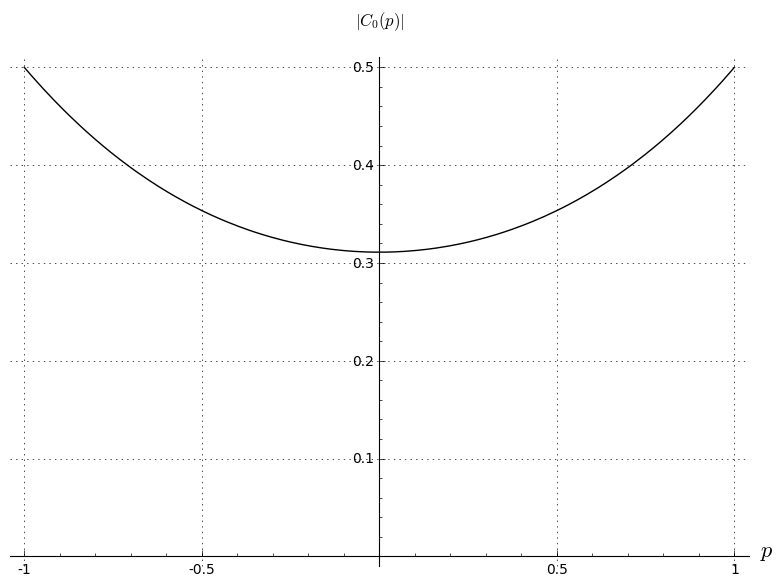
\includegraphics[width=0.7\linewidth]{C0_p.png}
  \caption{Plot of $|C_0(p)|$ for $-1 \leq p \leq 1$.}
\end{figure}

Informally, the above proposition (and \eqref{RON-def}, \eqref{M-def}) yield the approximation
\begin{align*}
 R_{0,N}(s) &\approx \frac{1}{8} \frac{s(s-1)}{2} \pi^{-s/2} \Gamma\left(\frac{s}{2}\right) (-1)^{N-1} U a^{-\sigma} C_0(p) \\
&\approx (-1)^{N-1} U M_0(s) a^{-\sigma} C_0(p).
\end{align*}
If one writes $s = \sigma+iT$, then by using the approximation $\alpha(s) \approx \frac{1}{2} \log \frac{iT}{2\pi}$ for the log-derivative of $M_0$, one can then obtain the approximate formula
$$ R_{0,N}(s) \approx (-1)^{N-1} U e^{\pi i \sigma/4} M_0(iT) C_p(p).$$
In fact we have the more general approximation
$$ R_{t,N}(s) \approx (-1)^{N-1} U e^{\pi i \sigma/4} \exp\left( \frac{t \pi^2}{64}\right) M_0(iT') C_p(p)$$
where $T' \coloneqq T + \frac{\pi t}{8}$.  More precisely, we have

\begin{proposition}[Estimate for $R_{t,N}$]\label{RTN-prop}  Let $0 \leq \sigma \leq 1$, let $T \geq 100$, and let $0 < t \leq 1/2$.  Set
$$ T' \coloneqq T + \frac{\pi t}{8} $$
and then define $a,N,p,U,C_0(p)$ using \eqref{a-def}, \eqref{N-def}, \eqref{U-def}, \eqref{C0-def}.
Then 
$$
 R_{t,N}(\sigma+iT) = (-1)^{N-1} U e^{\pi i \sigma/4} \exp\left( \frac{t \pi^2}{64}\right) M_0(iT') \left( C_0(p) + O_{\leq}( \tilde \eps(\sigma+iT))\right)$$
where
\begin{equation}\label{epsp-def}
 \tilde \eps(\sigma+iT) \coloneqq \left(\frac{0.397 \times 9^\sigma}{a-0.125} + \frac{5}{3(T'-3.33)}\right) \exp\left( \frac{3.49}{T'-3.33} \right).
\end{equation}
\end{proposition}

\begin{proof}  We apply \eqref{RTN-def} with $\beta_N := \pi i/4$ to obtain
$$ R_{t,N}(\sigma+iT) = \exp\left( \frac{t \pi^2}{64}\right) \int_\R \exp\left( - \frac{\sqrt{t} v \pi i}{4}\right) R_{0,N}( \sigma+iT' + \sqrt{t} v) \frac{1}{\sqrt{\pi}} e^{-v^2}\ dv.$$
From \eqref{RON-def} we have
$$ R_{0,N}( \sigma+iT' + \sqrt{t} v) = \frac{1}{8} \frac{s_v(s_v-1)}{2} \pi^{-s_v/2} \Gamma\left(\frac{s_v}{2}\right) (-1)^{N-1} U a^{-\sigma-\sqrt{t} v}
\left(\sum_{k=0}^{K_v} \frac{C_k(p,\sigma + \sqrt{t} v)}{a^k} + RS_{K_v}(s_v)\right) $$
for any positive integer $K_v$ that we permit to depend (in a measurable fashion) on $v$, where $s_v \coloneqq \sigma + iT' + \sqrt{t} v$. From \eqref{M-def} and Lemma \ref{elem-lem}(v) we thus have
$$ R_{0,N}( \sigma+iT' + \sqrt{t} v) = M_0(s_v) \exp\left( O_{\leq}\left(\frac{1}{12(T'-0.33)}\right) \right) (-1)^{N-1} U a^{-\sigma-\sqrt{t} v}
\left(\sum_{k=0}^{K_v} \frac{C_k(p,\sigma + \sqrt{t} v)}{a^k} + RS_{K_v}(s_v)\right).$$
From \eqref{alpha-deriv-bound} and Taylor expansion of the logarithm $\log M_0$ defined in \eqref{logM}, we have
$$ M_0(s_v) = M_0(iT') \exp\left( \alpha(iT') (\sigma + \sqrt{t} v) + O_{\leq}\left( \frac{(\sigma + \sqrt{t} v)^2}{4(T'-0.33)} \right) \right).$$
From \eqref{alpha-form}, \eqref{a-def} one has
$$ \alpha(iT') = O_{\leq}\left( \frac{1}{2T'}\right) + O_{\leq}\left( \frac{1}{T'}\right) + \frac{1}{2} \Log \frac{iT'}{2\pi} = \log a + \frac{i\pi}{4} + O_{\leq}\left( \frac{3}{2T'}\right)$$
and hence (bounding $\frac{3}{2T'}$ by $\frac{6}{4(T'-0.33)}$)
$$ \alpha(iT') (\sigma + \sqrt{t} v)  = (\sigma + \sqrt{t} v)  \log a + \frac{\pi i \sigma}{4} + \frac{\sqrt{t} v \pi i}{4} + O_{\leq}\left( \frac{6 |\sigma+\sqrt{t} v|}{4(T'-0.33)} \right).$$ 
We conclude that
\begin{align*}
\exp\left( - \frac{\sqrt{t} v \pi i}{4}\right) R_{0,N}( \sigma+iT' + \sqrt{t} v) &= 
M_0(iT') \exp\left( O_{\leq}\left(\frac{(\sigma + \sqrt{t} v)^2+6|\sigma+\sqrt{t} v|+\frac{1}{3}}{4(T'-0.33)} \right)\right) \times \\
&\quad \times (-1)^{N-1} U  e^{\pi i \sigma/4} \left(\sum_{k=0}^{K_v} \frac{C_k(p, \sigma+\sqrt{t} v)}{a^k} + RS_{K_v}(s_v)\right).
\end{align*}
Bounding $6|\sigma+\sqrt{t} v| \leq 3 (\sigma + \sqrt{t} v)^2 + 3$, we have
$$ \frac{(\sigma + \sqrt{t} v)^2+6|\sigma+\sqrt{t} v|+\frac{1}{3}}{4(T'-0.33)}  \leq \frac{(\sigma + \sqrt{t} v)^2 + \frac{5}{6}}{T'-0.33}.$$
Putting all this together, we obtain
\begin{align*}
 R_{t,N}(\sigma+iT) &= (-1)^{N-1} U e^{\pi i \sigma/4} \exp\left( \frac{t \pi^2}{64}\right) M_0(iT') \times \\
&\quad \times \int_\R \exp\left( O_{\leq}\left(\frac{(\sigma + \sqrt{t} v)^2 + \frac{5}{6}}{T'-0.33} \right) \right) \left(\sum_{k=0}^{K_v} \frac{C_k(p,\sigma + \sqrt{t} v)}{a^k} + RS_{K_v}(s_v)\right) \frac{1}{\sqrt{\pi}} e^{-v^2}\ dv.
\end{align*}
We separate the $k=0$ term from the rest.
By Lemma \ref{elem-lem}(iv) and the fact that $\frac{1}{\sqrt{\pi}} e^{-v^2}$ integrates to one, we can write the above expression as
\begin{equation}\label{rtnst}
 R_{t,N}(\sigma+iT) = (-1)^{N-1} U e^{\pi i \sigma/4} \exp\left( \frac{t \pi^2}{64}\right) M_0(iT') \left( C_0(p) (1 + O_{\leq}(\epsilon)) + O_{\leq}(\delta) \right)
\end{equation}
where
$$ \epsilon := \int_\R \left( \exp\left( \frac{(\sigma + \sqrt{t} v)^2 + \frac{5}{6} }{T'-0.33} \right)  - 1\right) \frac{1}{\sqrt{\pi}} e^{-v^2}\ dv$$
and
$$ \delta := \int_\R \exp\left( \frac{(\sigma + \sqrt{t} v)^2 + \frac{5}{6}}{T'-0.33} \right) \left(\sum_{k=1}^{K_v} \frac{|C_k(p,\sigma+\sqrt{t}v)|}{a^k} + |RS_{K_v}(s_v)|\right) \frac{1}{\sqrt{\pi}} e^{-v^2}\ dv.$$
Bounding $(\sigma + \sqrt{t} v)^2 \leq 2 \sigma^2 + 2 t v^2$ and using \eqref{gaussian} we obtain
$$ \epsilon \leq \exp\left( \frac{2\sigma^2 + \frac{5}{6}}{T'-0.33} \right) \left(1 - \frac{2t}{T'-0.33}\right)^{-1/2} - 1.$$
Applying Lemma \ref{elem-lem}(ii) and using the hypotheses $t \leq 1/2$, $T \geq 100$, one has
$$ 1 - \frac{2t}{T'-0.33} = \exp\left( O_{\leq}\left( \frac{2t}{T'-3.33} \right)\right)$$
and hence
$$
 \epsilon \leq \exp\left( \frac{2\sigma^2 + t + \frac{5}{6}}{T'-3.33} \right) - 1.
$$
With $t \leq 1/2$ and $0 \leq \sigma \leq 1$, one has $2\sigma^2 + t + \frac{5}{6} \leq \frac{10}{3}$.  By the mean value theorem we then have
\begin{equation}\label{eep}
 \epsilon \leq \frac{10}{3(T'-3.33)} \exp\left( \frac{10}{3(T'-3.33)}\right).
\end{equation}

Now we work on $\delta$.  Making the change of variables $u \coloneqq \sigma + \sqrt{t} v$, we have
$$ \delta = \int_\R \exp\left( \frac{u^2 + \frac{5}{6}}{T'-0.33} \right) \left(\sum_{k=1}^{\tilde K_u} \frac{|C_k(p,u)|}{a^k} + |RS_{\tilde K_u}(u + iT')|\right) \frac{1}{\sqrt{\pi t}} e^{-(u-\sigma)^2/t}\ du,$$
where $\tilde K_u$ is a positive integer parameter that can depend arbitrarily on $u$ (as long as it is measurable, of course).  

We choose $\tilde K_u$ to equal $1$ when $u \geq 0$ and $\max( \lfloor -\sigma \rfloor + 3, \lfloor \frac{T'}{\pi} \rfloor )$ when $u < 0$, so that Proposition \ref{arias-prop} applies.  The expression
$$ \sum_{k=1}^{\tilde K_u} \frac{|C_k(p,u)|}{a^k} + |RS_{\tilde K_u}(u + iT')| $$
is then bounded by
\begin{equation}\label{u0}
 \frac{\sqrt{2}}{2\pi} \frac{9^u \Gamma(1/2)}{2a} + \frac{1}{7} 2^{3u/2} \frac{\Gamma(1)}{(a/1.1)^2}
\leq \frac{0.200 \times 9^u}{a} + \frac{0.173 \times 2^{3u/2}}{a^2} 
\end{equation}
for $u \geq 0$ and
\begin{equation}\label{laf}
 \sum_{1 \leq k \leq \tilde K_u} \frac{2^{\frac{1}{2}-u}}{2\pi} \frac{\Gamma(k/2)}{2\pi ((3-2\log 2)\pi)^{k/2} a^k} + \frac{1}{2} (9/10)^{\lceil -u \rceil} \frac{\Gamma((\tilde K_u + 1)/2)}{(a/1.1)^{\tilde K_u + 1}}
\end{equation}
for $u < 0$.  One can calculate that
$$ \frac{2^{\frac{1}{2}}}{2\pi} \frac{1}{2\pi} \leq 0.036 \leq \frac{1}{2}$$
and
$$ \frac{1}{((3-2\log 2)\pi)^{1/2}} \leq 0.445 \leq 1.1$$
and hence we can bound \eqref{laf} by
$$  0.036 2^{-u} \sum_{1 \leq k \leq \frac{T'}{\pi}} (0.445)^k \frac{\Gamma(k/2)}{a^k} 
\frac{1}{2} 2^{-u} \sum_{\frac{T'}{\pi} \leq k \leq -u+4} \frac{\Gamma(k/2)}{(a/1.1)^k}.$$

For $u \geq 0$, we can estimate \eqref{u0} by
$$ 0.2 \times 9^u \left(\frac{1}{a} + \frac{0.865}{a^2}\right) \leq \frac{0.2 \times 9^u}{a - 0.865}$$
thanks to Lemma \ref{elem-lem}(i).  For $u<0$, we observe that if $k \leq 2 a^2 = \frac{T'}{\pi}$ then
$$ \frac{\Gamma(k+2/2)}{a^{k+2}} = \frac{k}{2 a^2} \frac{\Gamma(k/2)}{a^k} \leq \frac{\Gamma(k/2)}{a^k}$$
and hence by the geometric series formula
$$ \sum_{2 \leq k \leq \frac{T'}{\pi}, k\ \mathrm{even}} (0.445)^k \frac{\Gamma(k/2)}{a^k}  \leq \frac{(0.445)^2}{1-(0.445)^2} \frac{\Gamma(2/2)}{a} \leq \frac{0.247}{a^2}$$
and similarly
$$ \sum_{3 \leq k \leq \frac{T'}{\pi}, k\ \mathrm{odd}} (0.445)^k \frac{\Gamma(k/2)}{a^k}  \leq \frac{(0.445)^3}{1-(0.445)^2} \frac{\Gamma(3/2)}{(a/1.1)^3} \leq \frac{0.098}{a^3}$$
and hence we can bound \eqref{laf} by
$$ 0.036 2^{-u} \left(\frac{0.445 \sqrt{\pi}}{a} + \frac{0.247}{a^2} + \frac{0.098}{a^3}\right) + \frac{1}{2} 2^{-u}  \sum_{\frac{T'}{\pi} \leq k \leq -u+4} \frac{\Gamma(k/2)}{(a/1.1)^k}.$$
By Lemma \ref{elem-lem}(i) we have
$$ 0.036 \left(\frac{0.445 \sqrt{\pi}}{a} + \frac{0.247}{a^2} + \frac{0.098}{a^3}\right) \leq \frac{0.029}{a - 0.353}$$
and thus we can bound \eqref{laf} by
$$ \frac{0.029 \times 2^{-u}}{a - 0.353} + \frac{1}{2} 2^{-u} \sum_{\frac{T'}{\pi} \leq k \leq -u+4} (1.1)^{k} \frac{\Gamma(k/2)}{a^k}.$$

Putting this together, we conclude that
$$
\sum_{k=1}^{\tilde K_u} \frac{|C_k(p,u)|}{a^k} + |RS_{\tilde K_u}(u + iT')| \leq 
\frac{0.2 \times 9^u}{a-0.865} + \frac{0.029 \times 2^{-u}}{a - 0.353)} + \frac{2^{-u}}{2} \sum_{\frac{T'}{\pi} \leq k \leq -u+4} (1.1)^{k} \frac{\Gamma(k/2)}{a^k}$$
for all $u$ (positive or negative).  We conclude that $\delta \leq \delta_1 + \delta_2 + \delta_3$, where
\begin{align}
\delta_1 &\coloneqq \int_\R \exp\left( \frac{u^2 + \frac{5}{6}}{T'-0.33} \right) \frac{0.2 \times 9^u}{a-0.865} \frac{1}{\sqrt{\pi t}} e^{-(u-\sigma)^2/t}\ du \nonumber\\
\delta_2 &\coloneqq \int_\R \exp\left( \frac{u^2 + \frac{5}{6}}{T'-0.33} \right) \frac{0.029 \times 2^{-u}}{a - 1.25} \frac{1}{\sqrt{\pi t}} e^{-(u-\sigma)^2/t}\ du \nonumber\\
\delta_3 &\coloneqq \int_\R \exp\left( \frac{u^2 + \frac{5}{6}}{T'-0.33} \right) \frac{2^{-u}}{2} \sum_{\frac{T'}{\pi} \leq k \leq -u+4} (1.1)^{k} \frac{\Gamma(k/2)}{a^k} \frac{1}{\sqrt{\pi t}} e^{-(u-\sigma)^2/t}\ du.\label{delta3-def}
\end{align}
For $\delta_1$, we translate $u$ by $\sigma$ to obtain
$$ \delta_1 = \frac{0.2 \times 9^\sigma}{a-0.865} \int_\R \exp\left( \frac{u^2 + 2 \sigma u + \sigma^2 + \frac{5}{6}}{T'-0.33}  + 2 u \log 3 \right) \frac{1}{\sqrt{\pi t}} e^{-u^2/t}\ du$$
and hence by \eqref{gaussian}
\begin{equation}\label{delta1}
 \delta_1 = \frac{0.2 \times 9^\sigma}{a-0.865} \exp\left( \frac{\sigma^2 + \frac{5}{6}}{T'-0.33} + \frac{t(\log 3 + \frac{\sigma}{T'-0.33})^2}{1 - \frac{t}{T'-0.33}} \right) \left(1 - \frac{t}{T'-0.33}\right)^{-1/2}.
\end{equation}
One can write
\begin{equation}\label{hit}
 \frac{1}{1 - \frac{t}{T'-0.33}} = 1 + \frac{t}{T'-0.33-t} \leq 1 + \frac{t}{T'-0.83}
\end{equation}
while by Lemma \ref{elem-lem}(ii) we have
\begin{equation}\label{hit2}
 1 - \frac{t}{T'-0.33} = \exp\left( O_{\leq}\left( \frac{t}{T'-0.33-t} \right) \right) = \exp\left( O_{\leq}\left( \frac{t}{T'-0.83} \right) \right).
\end{equation}
We conclude that
$$ \delta_1 \leq \frac{0.2 \times 9^\sigma}{a-0.865} \exp\left( \frac{5+3t+6\sigma^2}{6(T'-0.83)} + t\left(\log 3 + \frac{\sigma}{T'-0.33}\right)^2 \left(1 + \frac{t}{T'-0.83}\right) \right).$$
From Lemma \ref{elem-lem}(i) and the hypothesis $0 \leq \sigma \leq 1$, we have
\begin{align*}
\left(\log 3 + \frac{\sigma}{T'-0.33}\right)^2 &\leq (\log^2 3) \left(1 + \frac{2 \sigma / \log 3}{T' - 0.33 - \frac{\sigma}{2\log 3}}\right) \\
&\leq  (\log^2 3) \left(1 + \frac{2 \sigma / \log 3}{T' - 0.83}\right)
\end{align*}
and therefore by a further application of Lemma \ref{elem-lem}(i)
\begin{align*}
\left(\log 3 + \frac{\sigma}{T'-0.33}\right)^2 \left(1 + \frac{t}{T'-0.83}\right) 
&\leq \log^2 3 \left(1 + \frac{\frac{2 \sigma}{\log 3} + t}{T' - 0.83 - \frac{2\sigma t/\log 3}{2\sigma/\log 3 + t}}\right) \\
&\leq \log^2 3 \left(1 + \frac{\frac{2 \sigma}{\log 3} + t}{T' - 0.83 - t}\right) \\
&\leq \log^2 3 \left(1 + \frac{\frac{2 \sigma}{\log 3} + t}{T' - 1.33}\right) 
\end{align*}
and thus
$$ \delta_1 \leq \frac{0.2 \times 9^\sigma \exp( t \log^2 3 )}{a-0.865} \exp\left( \frac{5+3t+6\sigma^2 + 12 t \sigma \log 3 + 6t^2 \log^2 3}{6(T'-1.33)} \right).$$

By repeating the proof of \eqref{delta1}, we have
$$
 \delta_2 = \frac{0.029 \times 2^{-\sigma}}{a - 0.353} \exp\left( \frac{\sigma^2 + \frac{5}{6}}{T'-0.33} + \frac{t\left(-\log \sqrt{2} + \frac{\sigma}{T'-0.33}\right)^2}{1 - \frac{t}{T'-0.33}} \right) \left(1 - \frac{t}{T'-0.33}\right)^{-1/2}.$$
We can bound $(-\log \sqrt{2} + \frac{\sigma}{T'-0.33})^2$ by $\log^2 \sqrt{2}$.  Using \eqref{hit}, \eqref{hit2} we thus have
$$
 \delta_2 \leq \frac{0.029 \times 2^{-\sigma} \exp( t \log^2 \sqrt{2})}{a - 0.353} \exp\left( \frac{5 + 3t + 6\sigma^2}{6(T'-1.33)} \right).
$$

With $t \leq 1/2$ and $0 \leq \sigma \leq 1$ one has
\begin{align*}
 0.2 \exp(t \log^2 3) &\leq 0.366 \\
0.029 \exp( t \log^2 \sqrt{2}) &\leq 0.031 \\
\frac{5 + 3t + 6\sigma^2}{6} \leq \frac{5 + 3t + 6\sigma^2 + 12 t \sigma \log 3 + 6t^2 \log^2 3}{6} &\leq 3.49
\end{align*}
and hence
$$ \delta_1 \leq \frac{0.366 \times 9^\sigma}{a-0.865} \exp\left( \frac{3.49}{T'-1.33} \right)$$
and
$$ \delta_2 \leq \frac{0.031 \times 2^{-\sigma}}{a-0.353} \exp\left( \frac{3.49}{T'-1.33} \right).$$

Now we turn to $\delta_3$, which will end up being extremely small compared to $\delta_1$ or $\delta_2$. By \eqref{delta3-def} and the Fubini-Tonelli theorem, we have
$$ \delta_3 = \frac{1}{2 \sqrt{\pi t}} \sum_{k \geq \frac{T'}{2.2 \pi}} (1.1)^{k} \frac{\Gamma(k/2)}{a^k} \int_{-\infty}^{4-k} \exp\left( \frac{u^2 + \frac{5}{6}}{T'-0.33}  - \frac{(u-\sigma)^2}{t} - u \log 2\right)\ du.$$
Since $u \leq 4-k$, $k \geq \frac{T'}{2.2\pi}$, and $T' \geq T \geq 100$, we have $k \geq 14$ and $u \leq -10$; since $\sigma \geq 0$, we may thus lower bound $(u-\sigma)^2/t$ by $u^2/t$.  Since $t \leq 1/2$, we can upper bound $\frac{u^2 + \frac{5}{6}}{T'-0.33} - \frac{u^2}{t}$ by (say) $-\frac{u^2}{2t}$, thus
$$ \delta_3 \leq \frac{1}{2 \sqrt{\pi t}} \sum_{k \geq \frac{T'}{2.2 \pi}} (1.1)^{k} \frac{\Gamma(k/2)}{a^k} \int_{-\infty}^{4-k} e^{-\frac{u^2}{2t} - u \log 2}\ du.$$
We can bound $e^{-\frac{u^2}{2t}} \leq e^{\frac{(k-4)u}{2t}}$, in the range of integration and thus
$$ \int_{-\infty}^{4-k} e^{-\frac{u^2}{2t} - u \log 2}\ du \leq \frac{1}{\frac{k-4}{2t} - \log 2} e^{-\frac{(k-4)^2}{2t} + (k-4) \log 2} \leq \frac{1}{\frac{k-4}{2t} - \log 2} e^{-(k-4)^2 + (k-4) \log 2};$$
bounding
$$ \frac{k-4}{2t} - \log 2 = \frac{k-4-2t \log 2}{2t} \geq \frac{k-6}{2t}$$
we conclude that
$$ \delta_3 \leq \frac{\sqrt{t}}{\sqrt{\pi}} \sum_{k \geq \frac{T'}{2.2 \pi}} (1.1)^{k} \frac{\Gamma(k/2)}{(k-6) a^k} e^{-(k-4)^2 + (k-4) \log 2}.$$
For $k \geq 14$ one can easily verify that $(1.1)^{k} \Gamma(k/2) e^{-(k-4)^2 + (k-4) \log 2} \leq 10^{-30}$; discarding the $\frac{\sqrt{t}}{\sqrt{\pi}}$ and $\frac{1}{k-6}$ factors we thus have
$$ \delta_3 \leq \sum_{k \geq 14} \frac{10^{-30}}{a^k} \leq \frac{2 \times 10^{-30}}{a^{14}}$$
(say).   Since
$$ \frac{0.031 \times 2^{-\sigma}}{a-0.353} + \frac{2 \times 10^{-30}}{a^{14}} \leq \frac{0.031 \times 2^{-\sigma}}{a-0.865}$$
we thus have
$$ \delta \leq \delta_1+\delta_2+\delta_3 \leq \frac{0.366 \times 9^\sigma + 0.031 \times 2^{-\sigma}}{a-0.865} \exp\left( \frac{3.49}{T'-1.33} \right).$$
Inserting this and \eqref{eep}, \eqref{cop} into \eqref{rtnst}, and crudely bounding $2^{-\sigma}$ by $9^\sigma$, we obtain the claim.
\end{proof}

\subsection{Combining the estimates}


Combining Propositions \ref{rtn-prop}, \ref{RTN-prop} with \eqref{htz-expand} and the triangle inequality (and noting that $M_0 = M_0^*$, $M_t = M_t^*$ and $\alpha = \alpha^*$, and that $U$ has magnitude $1$), we conclude the following ``$A+B-C$ approximation to $H_t$'':

\begin{corollary}[$A+B-C$ approximation]\label{abc-cor}  Let $t,x,y$ obey \eqref{region}.  Set
\begin{equation}\label{tp-def}
 T' \coloneqq \frac{x}{2} + \frac{\pi t}{8} 
\end{equation}
and then define $a,N,p,U,C_0(p)$ using \eqref{a-def}, \eqref{N-def}, \eqref{U-def}, \eqref{C0-def}.  Define the quantities
\begin{align*}
A(x+iy) &\coloneqq M_t(\frac{1-y+ix}{2}) \sum_{n=1}^N \frac{b_n^t}{n^{\frac{1-y+ix}{2}  +\frac{t}{2} \alpha(\frac{1-y+ix}{2})}}  \\
B(x+iy) &\coloneqq M_t(\frac{1+y-ix}{2}) \sum_{n=1}^N \frac{b_n^t}{n^{\frac{1+y-ix}{2} +\frac{t}{2} \alpha(\frac{1+y-ix}{2})}}  \\
C(x+iy) &\coloneqq  2 e^{-\pi i y/8} (-1)^{N} \exp\left( \frac{t \pi^2}{64}\right) \mathrm{Re}( M_0(iT') C_0(p) U e^{\pi i/8} )
\end{align*}
where $M_0, b_n^t$ were defined in \eqref{Mt-def}, \eqref{bn-def}.
Then
$$ H_t(x+iy) = A(x+iy) + B(x+iy) - C(x+iy) + O_{\leq}(E_A(x+iy) + E_B(x+iy) + E_C(x+iy))$$
where
\begin{align*}
E_A(x+iy) &\coloneqq \left|M_t\left(\frac{1-y+ix}{2}\right)\right| \sum_{n=1}^N \frac{b_n^t}{n^{\frac{1-y}{2}+\frac{t}{2} \mathrm{Re} \alpha(\frac{1-y+ix}{2})}} \eps_{t,n}(\frac{1-y+ix}{2}) \\
E_B(x+iy) &\coloneqq \left|M_t\left(\frac{1+y+ix}{2}\right)\right|\sum_{n=1}^N  \frac{b_n^t}{n^{\frac{1+y}{2}+\frac{t}{2} \mathrm{Re} \alpha(\frac{1+y+ix}{2})}} \eps_{t,n}(\frac{1+y+ix}{2})  \\
E_C(x+iy) &\coloneqq \exp\left( \frac{t \pi^2}{64}\right) |M_0(iT')| \left(\tilde \eps(\frac{1-y+ix}{2}) + \tilde \eps(\frac{1+y+ix}{2})\right)  
\end{align*}
and $\eps_{t,n}, \tilde \eps$ were defined in \eqref{eps-def}, \eqref{epsp-def}. 
\end{corollary}

In our applications, we will just use the cruder ``$A+B$'' approximation that is immediate from the above corollary and \eqref{cop}:

\begin{corollary}[$A+B$ approximation]\label{ab-cor} With the notation and hypotheses as in Corollary \ref{abc-cor}, we have
$$ H_t(x+iy) = A(x+iy) + B(x+iy) + O_{\leq}(E_A(x+iy) + E_B(x+iy) + E_{C,0}(x+iy))$$
where
\begin{align*}
E_{C,0}(x+iy) &\coloneqq \exp\left( \frac{t \pi^2}{64}\right) |M_0(iT')| \left(1 + \tilde \eps\left(\frac{1-y+ix}{2}\right) + \tilde \eps\left(\frac{1+y+ix}{2}\right)\right). 
\end{align*}
\end{corollary}

We can now prove Theorem \ref{eff}.  Dividing by the expression $B_0$ from \eqref{bo-def}, and using \eqref{ft-def}, we conclude that
\begin{equation}\label{ratio-form-refined}
\frac{H_t(x+iy)}{B_0(x+iy)} = f_t(x+iy) + \frac{C(x+iy)}{B_0(x+iy)} + O_{\leq}\left( e_A + e_B + e_{C} \right)
\end{equation}
and
\begin{equation}\label{ratio-form}
\frac{H_t(x+iy)}{B_0(x+iy)} = f_t(x+iy) + O_{\leq}\left( e_A + e_B + e_{C,0} \right)
\end{equation}
where
\begin{align}
e_A \coloneqq e_A(x+iy) &\coloneqq |\gamma| \sum_{n=1}^N n^y \frac{b_n^t}{n^{\mathrm{Re}(s) + \mathrm{Re}(\kappa)}} \eps_{t,n}\left(\frac{1-y+ix}{2}\right) \label{ea-def}\\
e_B \coloneqq e_B(x+iy) &\coloneqq \sum_{n=1}^N  \frac{b_n^t}{n^{\mathrm{Re}(s)}} \eps_{t,n}\left(\frac{1+y+ix}{2}\right) \label{eb-def} \\
e_{C} \coloneqq e_{C}(x+iy) &\coloneqq \frac{\exp\left( \frac{t \pi^2}{64}\right) |M_0(iT')|}{|M_t(\frac{1+y+ix}{2})|} \left(\tilde \eps\left(\frac{1-y+ix}{2}\right) + \tilde \eps\left(\frac{1+y+ix}{2}\right)\right).\label{ecc-def}\\
e_{C,0} \coloneqq e_{C,0}(x+iy) &\coloneqq \frac{\exp\left( \frac{t \pi^2}{64}\right) |M_0(iT')|}{\left|M_t\left(\frac{1+y+ix}{2}\right)\right|} \left(1 + \tilde \eps\left(\frac{1-y+ix}{2}\right) + \tilde \eps\left(\frac{1+y+ix}{2}\right)\right),\label{ec-def}
\end{align}
and where $\gamma,s_*,\kappa$ were defined in \eqref{lambda-def}, \eqref{sn-def}, \eqref{kappa-def}.  Note also from \eqref{tp-def}, \eqref{a-def}, \eqref{N-def} that $N$ is given by \eqref{N-def-main}.

To conclude the proof of Theorem \ref{eff} it thus suffices to obtain the following estimates.

\begin{proposition}[Estimates]\label{estimates}  Let the notation and hypotheses be as above. 
\begin{itemize}
\item[(i)]  One has
$$ |\gamma| \leq e^{0.02 y} \left( \frac{x}{4\pi} \right)^{-y/2} $$
\item[(ii)] One has
$$ \mathrm{Re} s_* \geq \frac{1+y}{2} +\frac{t}{4} \log \frac{x}{4\pi} - \frac{(1-3y+\frac{4y(1+y)}{x^2})_+ t}{2x^2}.$$
\item[(iii)]  One has
$$ \kappa = O_{\leq} \left( \frac{ty}{2(x-6)} \right).$$
\item[(iv)]  One has
$$ e_A \leq |\gamma| N^{|\kappa|} \sum_{n=1}^N n^{y} \frac{b_n^t}{n^{\mathrm{Re}(s_*)}} \left( \exp\left( \frac{\frac{t^2}{16} \log^2 \frac{x}{4\pi n^2} + 0.626}{\frac{x}{2}-6.66} \right)-1 \right).$$
\item[(v)]  One has
$$ e_B \leq \sum_{n=1}^N  \frac{b_n^t}{n^{\mathrm{Re}(s_*)}} \left( \exp\left( \frac{\frac{t^2}{16} \log^2 \frac{x}{4\pi n^2} + 0.626}{x-6.66} \right)-1 \right).$$
\item[(vi)] One has
$$ e_{C} \leq \left(\frac{x}{4\pi}\right)^{-\frac{1+y}{4}} \exp\left( - \frac{t}{16} \log^2 \frac{x}{4\pi} + \frac{3 |\log \frac{x}{4\pi} + i \frac{\pi}{2}|+3.58}{x-8.52} \right) \left(\frac{1.24 \times (3^y+3^{-y})}{N-0.125} + \frac{6.92}{x-6.66}\right).
$$
and
$$ e_{C,0} \leq \left(\frac{x}{4\pi}\right)^{-\frac{1+y}{4}} \exp\left( - \frac{t}{16} \log^2 \frac{x}{4\pi} + \frac{3 |\log \frac{x}{4\pi} + i \frac{\pi}{2}|+3.58}{x-8.52} \right) \left(1 + \frac{1.24 \times (3^y+3^{-y})}{N-0.125} + \frac{6.92}{x-6.66}\right).
$$
\end{itemize}
\end{proposition}

Note that to obtain the bound \eqref{ec-bound} from Proposition \ref{estimates}(vi) we may simply use the inequality $1+u \leq \exp(u)$ for any $u \in \R$, and then bound $\frac{1}{x-6.66} \leq \frac{1}{x-8.52}$.

\begin{proof}
From the mean value theorem (and noting that $M_t = M_t^*$, so that $\left|M_t\left(\frac{1+y-ix}{2}\right)\right| = \left|M_t\left(\frac{1+y+ix}{2}\right)\right|$), we have
$$ \log|\gamma| = -y \frac{d}{d\sigma} \log \left|M_t\left( \sigma + \frac{ix}{2}\right)\right| $$
for some $\frac{1-y}{2} \leq \sigma \leq \frac{1+y}{2}$.  From \eqref{alpha-def}, \eqref{Mt-def} we have
$$ \frac{d}{d\sigma} \log \left|M_t\left( \sigma + \frac{ix}{2}\right)\right| = \mathrm{Re}\left( \frac{t}{2} \alpha\left(\sigma+\frac{ix}{2}\right) \alpha'\left(\sigma+\frac{ix}{2}\right) + \alpha\left(\sigma+\frac{ix}{2}\right) \right).$$
From \eqref{alpha-deriv-bound} one has
\begin{equation}\label{alphap-b}
 \alpha'\left(\sigma+\frac{ix}{2}\right) = O_{\leq}\left( \frac{1}{x-6} \right)
\end{equation}
and from Taylor expansion we also have
$$ \alpha(\sigma+\frac{ix}{2}) = \alpha\left(\frac{ix}{2}\right) + O_{\leq}\left( \frac{\sigma}{x-6} \right);$$
from \eqref{alpha-form} one has
$$ \alpha\left(\frac{ix}{2}\right) = O_{\leq}\left(\frac{1}{x}\right) + O_{\leq}\left(\frac{1}{x}\right) + \frac{1}{2} \Log \frac{ix}{4\pi} 
= \frac{1}{2} \log \frac{x}{4\pi} + i \frac{\pi}{4} + O_{\leq}\left( \frac{2}{x} \right) $$
and hence
\begin{equation}\label{asig}
 \alpha(\sigma+\frac{ix}{2}) = \frac{1}{2} \log \frac{x}{4\pi} + i \frac{\pi}{4} + O_{\leq}\left( \frac{2+\sigma}{x-6} \right).
\end{equation}
Inserting these bounds, we conclude that
$$ \log|\gamma| = -y \mathrm{Re} \left( \left(\frac{1}{2} \log \frac{x}{4\pi} + i \frac{\pi}{4} + O_{\leq}\left( \frac{2+\sigma}{x-6} \right)\right) \left(1 + O_{\leq}\left(\frac{t}{2(x-6)}\right)\right) \right).$$
Expanding this out, we have
$$ \log|\gamma| = -y (\frac{1}{2} \log \frac{x}{4\pi} + O_{\leq}\left( \frac{2+\sigma + \frac{t}{4} \log \frac{x}{4\pi} + \frac{t\pi}{8} + \frac{t(2+\sigma)}{2(x-6)}}{x-6} \right)).$$
In the region \eqref{region}, which implies that $0 \leq \sigma \leq 1$, we have
$$ 2 + \sigma + \frac{t\pi}{8} + \frac{t(2+\sigma)}{2(x-6)} \leq 3.21$$
and thus
$$ \log|\gamma| \leq -\frac{y}{2} \log \frac{x}{4\pi} + y \frac{\frac{t}{4} \log \frac{x}{4\pi} + 3.21}{x-6}.$$
The function $x \mapsto \frac{\log \frac{x}{4\pi}}{x-6}$ is decreasing for $x \geq 200$ thanks to Lemma \ref{elem-lem}(vi), hence
$$ y \frac{\frac{t}{4} \log \frac{x}{4\pi} + 3.21}{x-6} \leq y \frac{\frac{t}{4} \log \frac{200}{4\pi} + 3.21}{200-6} \leq 0.02 y.$$
Claim (i) follows.  We remark that one can improve the $e^{0.02 y}$ factor here by Taylor expanding $\alpha$ to second order rather than first order, but we will not need to do so here.

To prove claim (ii), it suffices by \eqref{s-def} to show that
$$ \mathrm{Re} \alpha\left(\frac{1+y-ix}{2}\right) \geq \frac{1}{2} \log \frac{x}{4\pi} - \frac{(1-3y)_+}{x^2} - \frac{4y(1+y)}{x^4}.$$
By \eqref{alpha-form} one has
$$ \mathrm{Re} \alpha\left(\frac{1+y-ix}{2}\right) = \frac{1+y}{(1+y)^2+x^2} - \frac{2(1-y)}{(1-y)^2+x^2} + \frac{1}{2} \log \frac{\sqrt{(1+y)^2+x^2}}{4\pi}.$$
We bound $\sqrt{(1+y)^2+x^2} \geq x$ and calculate
\begin{align*}
 \frac{1+y}{(1+y)^2+x^2} - \frac{2(1-y)}{(1-y)^2+x^2} &= - \frac{1-3y}{(1+y)^2+x^2} -\frac{4y(1+y)}{((1+y)^2+x^2)((1+y)^2+x^2)} \\
&\geq - \frac{1-3y+\frac{4y(1+y)}{x^2}}{(1+y)^2+x^2}.
\end{align*}
Lower bounding the numerator by its nonnegative part and then lower bounding $(1+y)^2+x^2$ by $x^2$, we obtain the claim.

Claim (iii) is immediate from \eqref{alphap-b} and the fundamental theorem of calculus.  Now we turn to (iv), (v).  From \eqref{asig} one has
$$ \alpha\left(\frac{1 \pm y + ix}{2}\right) - \log n = \frac{1}{2} \log \frac{x}{4\pi n^2} + i \frac{\pi}{4} + O_{\leq}\left( \frac{3}{x-6}\right)$$
for either choice of sign $\pm$.  In particular, we have
\begin{equation}\label{alphn}
 \left|\alpha\left(\frac{1 \pm y + ix}{2}\right) - \log n\right|^2 = \frac{1}{4} \log^2 \frac{x}{4\pi n^2} + \frac{\pi^2}{16} + 
O_{\leq}\left( \frac{3 |\log \frac{x}{4\pi n^2} + i \frac{\pi}{2}|}{x-6} + \frac{9}{(x-6)^2}\right).
\end{equation}
For any $1 \leq n \leq N$, we have
$$ 1 \leq n^2 \leq N^2 \leq a^2 = \frac{x+\frac{\pi t}{16}}{4\pi};$$
in the region \eqref{region}, the right-hand side is certainly bounded by $(\frac{x}{4\pi})^2$, so that
$$ \frac{4\pi}{x} \leq \frac{x}{4\pi n^2} \leq \frac{x}{4\pi}$$
and hence
$$ \left|\log \frac{x}{4\pi n^2} + i \frac{\pi}{2}\right| \leq \left|\log \frac{x}{4\pi} + i \frac{\pi}{2}\right|.$$
In the region \eqref{region} we have  $x \geq 200$, we see from Lemma \ref{elem-lem}(vi) (after squaring) that $\frac{|\log \frac{x}{4\pi} + i \frac{\pi}{2}|}{x-6}$ is decreasing in $x$.  Thus
\begin{align*}
\frac{\pi^2}{16} + \frac{3 |\log \frac{x}{4\pi n^2} + i \frac{\pi}{2}|}{x-6} + \frac{9}{(x-6)^2}
&\leq \frac{\pi^2}{16} +  \frac{3 |\log \frac{200}{4\pi} + i \frac{\pi}{2}|}{200-6} + \frac{9}{(200-6)^2} \\
&\leq 0.667.
\end{align*}
Similarly, in \eqref{region} we also have
$$ \frac{t^2}{8} \times 0.667 + \frac{t}{4} + \frac{1}{6} \leq 0.313.$$ 
We conclude from \eqref{eps-def} that
$$
\eps_{t,n}\left(\frac{1 \pm y + ix}{2} \right) \leq \exp\left( \frac{\frac{t^2}{32} \log^2 \frac{x}{4\pi n^2} + 0.313}{T-3.33} \right)-1.$$
Inserting this bound into \eqref{ea-def}, \eqref{eb-def}, we obtain claims (iv), (v).

Now we establish (vi).  From \eqref{Mt-def} we have
$$\frac{\exp\left( \frac{t \pi^2}{64}\right) |M_0(iT')|}{|M_t(\frac{1+y+ix}{2})|}
= \exp\left( \frac{t \pi^2}{64} - \frac{t}{4} \mathrm{Re} \alpha\left(\frac{1+y+ix}{2}\right)^2\right) \frac{|M_0(iT')|}{|M_0\left(\frac{1+y+ix}{2}\right)|}.$$
Note that $\frac{1+y+ix}{2} = iT' + \frac{1+y}{2} - \frac{\pi i t}{8}$.  From \eqref{alpha-deriv-bound} we see that $|\alpha'(s)| \leq \frac{1}{x-6}$ for any $s$ on the line segment between $iT'$ and $\frac{1+y+ix}{2}$.  From Taylor's theorem with remainder applied to a branch of $\log M_0$, we conclude that
$$ \frac{|M_0(iT')|}{|M_0(\frac{1+y+ix}{2})|} = \exp\left( \mathrm{Re}\left( \left(-\frac{1+y}{2}+\frac{\pi i t}{8}\right) \alpha(iT') \right) + O_{\leq}\left( \frac{|-\frac{1+y}{2}+\frac{\pi i t}{8}|^2}{2(x-6)} \right) \right).$$
For $0 \leq y \leq 1$ and $0 < t \leq \frac{1}{2}$ we have
$$\frac{|-\frac{1+y}{2}+\frac{\pi i t}{8}|^2}{2} \leq 0.52$$
and from \eqref{alpha-form} one has
$$ \alpha(iT') = O_{\leq}\left(\frac{1}{2T'}\right) +  O_{\leq}\left(\frac{1}{T'}\right) + \frac{1}{2} \Log \frac{iT'}{2\pi} = \frac{1}{2} \log \frac{T'}{2\pi} + \frac{i\pi}{4} + O_{\leq}( \frac{3}{2T'} ) $$
and hence
$$
\frac{|M_0(iT')|}{|M_0\left(\frac{1+y+ix}{2}\right)|}
= \exp\left( -\frac{1+y}{4} \log \frac{T'}{2\pi} - \frac{t\pi^2}{32} + O_{\leq}\left( \frac{3|-\frac{1+y}{2}+\frac{\pi i t}{8}|}{2T'} + \frac{0.52}{x-6} \right) \right).$$
Bounding $\frac{1}{2T'} \leq \frac{1}{x-6}$ and $|-\frac{1+y}{2}+\frac{\pi i t}{8}| \leq 1.02$, this becomes
$$
\frac{|M_0(iT')|}{|M_0\left(\frac{1+y+ix}{2}\right)|}
= \left(\frac{T'}{2\pi}\right)^{-\frac{1+y}{4}} \exp\left( - \frac{t\pi^2}{32} + O_{\leq}\left( \frac{3.58}{x-6} \right) \right)$$
and hence
$$\frac{\exp\left( \frac{t \pi^2}{64}\right) |M_0(iT')|}{|M_t(\frac{1+y+ix}{2})|} 
= \left(\frac{T'}{2\pi}\right)^{-\frac{1+y}{4}} \exp\left( - \frac{t \pi^2}{64} - \frac{t}{4} \mathrm{Re} \alpha\left(\frac{1+y+ix}{2}\right)^2 + O_{\leq}\left( \frac{3.58}{x-6} \right) \right).$$
By repeating the proof of \eqref{alphn} we have
$$
\mathrm{Re} \alpha(\frac{1 \pm y + ix}{2})^2 = \frac{1}{4} \log^2 \frac{x}{4\pi} - \frac{\pi^2}{16} + 
O_{\leq}\left( \frac{3 |\log \frac{x}{4\pi} + i \frac{\pi}{2}|}{x-6} + \frac{9}{(x-6)^2}\right).
$$
As before, in the region \eqref{region} we have
$$\frac{3 |\log \frac{x}{4\pi n^2} + i \frac{\pi}{2}|}{x-6} + \frac{9}{(x-6)^2} \leq \frac{3 |\log \frac{x}{4\pi} + i \frac{\pi}{2}|}{x-6} + \frac{9}{(x-6)^2}
$$
and thus
\begin{align*}
\frac{\exp\left( \frac{t \pi^2}{64}\right) |M_0(iT')|}{\left|M_t\left(\frac{1+y+ix}{2}\right)\right|}
&= \left(\frac{T'}{2\pi}\right)^{-\frac{1+y}{4}} \exp\left( - \frac{t}{16} \log^2 \frac{x}{4\pi} + O_{\leq}\left( \frac{3 |\log \frac{x}{4\pi} + i \frac{\pi}{2}|+3.58}{x-6} + \frac{9}{(x-6)^2} \right) \right)\\
&= \left(\frac{T'}{2\pi}\right)^{-\frac{1+y}{4}} \exp\left( - \frac{t}{16} \log^2 \frac{x}{4\pi} + O_{\leq}\left( \frac{3 |\log \frac{x}{4\pi} + i \frac{\pi}{2}|+3.58}{x-8.52} \right) \right)
\end{align*}
thanks to Lemma \ref{elem-lem}(i).  Finally, since $T' \geq \frac{x}{2} \geq 100$ in \eqref{region}, one has 
$$\exp\left(\frac{3.49}{T'-3.33}\right) \leq 1.037$$
and hence by \eqref{epsp-def}
$$ 
\tilde \eps(\frac{1 \pm y+ix}{2}) \leq \frac{1.24 \times 3^{\pm y}}{a-0.125} + \frac{1.73}{T'-3.33}.$$
Hence
$$
\tilde \eps(\frac{1-y+ix}{2}) + \tilde \eps(\frac{1+y+ix}{2}) \leq \frac{1.24 \times (3^y+3^{-y})}{a-0.125} + \frac{3.46}{T'-3.33}$$
giving the claim (substituting $T' = x/2$ and $a \geq N$).
\end{proof}

{\bf give table illustrating accuracy of approximation}